\subsection*{Task 5.1}

A basis spline of order 1 is defined by:

\begin{align*}
	N_{i,1}(t) &= 
	\begin{cases}
	1, \text{if } t_i \le t < t_{i+1} \\
	0, \text{else} 
	\end{cases}
\end{align*}

For degrees $k > 1$ the b-spline is defined by the recursive function:

\begin{align*}
	N_{i,k}(t) &= \frac{t-t_i}{t_{i+k-1}-t_i}N_{i,k-1}(t)+\frac{t_{i+k}-t}{t_{i+k}-t_{i+1}}N_{i+1,k-1}(t)
\end{align*}

Figure \ref{fig:bspline} displays the basis splines of order 1 to 4. Note that only some time values are calculated and the intermediate values are interpolated. The b-spline of order 1 should be a perfect step function.
\begin{figure}[h]
	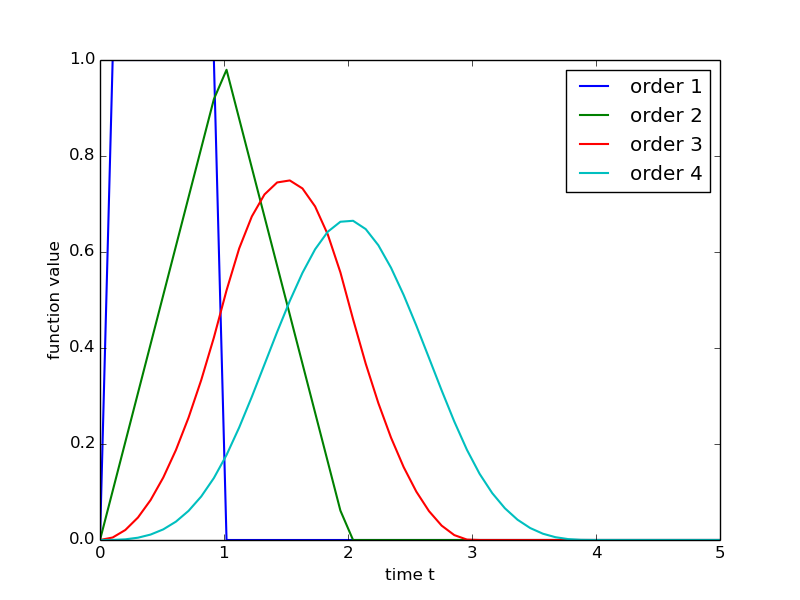
\includegraphics[scale=0.7]{Task_5_1.png}
	\caption{Basis splines of order 1 to 4 in time segment $t_0$ to $t_5$}
	\label{fig:bspline}
\end{figure}